\section{Background}\label{section2}

\subsection{Software Product Lines}

A Software Product Line (SPL) enables the creation of software-intensive systems that share and manage a set of features for satisfying the specific needs of a particular domain. Commonalities are shared by all derived products, while variabilities represent the scope of customization supported by them \cite{clements02,bockle05,vanderlinden07}.

The concept of SPL is suitable for domains in which products that share common features and a well-defined set of variabilities are demanded. At its essence, the conception of an SPL involves domain engineering and product development, both under technical and organizational management perspectives \cite{bockle05,vanderlinden07}.

The variabilities can be initially identified and represented by means of features, relevant and visible characteristics to stakeholders of a particular domain \cite{bosch01}. The precise and explicit representation and management of variabilities enable a consistent generation of specific products in an SPL \cite{chen11,galster2014}. 

According to \cite{bosch01}, the advantage of this model is that it allows for effective sharing of assets, i.e. software architectures and components, between a number of organizational units. On the other hand, the main disadvantage is that, due to the natural focus of the business units on systems (or products), there is no entity or explicit incentive to focus on the shared assets. This is the underlying cause for the erosion of the architecture and components in the system family. The timely and reliable evolution of the shared assets relies on the organizational culture and people commitment.

\subsection{SMarty: an Approach for Variability Management}

The proper management of variabilities has great relevance to ensure that all the benefits of SPL are obtained. Therefore, different approaches related to the variability management have been proposed by the research community. According to \cite{chen11}, Feature-oriented domain analysis (FODA) method, which was published in 1990, is one of the first contributions to variability management. Since then, a large number of effort has been spent on developing approaches for better managing variability.

In this context, SMarty is a variability management approach composed of a UML 2.4 profile (SMartyProfile) and supported by a systematic process (SMartyProcess), related to the main SPL activities \cite{oliveirajr10}. SMartyProcess defines a set of guidelines that supports the application of stereotypes and tagged-values. The guidelines ensure the identification and representation of variabilities and enabled the evolution of SPL, whereas the process incrementally and iteratively guarantees the identification of new variabilities and evolution of the SPL core assets.

The UML diagrams supported by SMarty (use case, class, sequence, component and activity) represent the static and dynamic aspects of software products. The SMarty effectiveness in identifying and representing variabilities in the UML models has been experimentally evaluated \cite{marcolino13,marcolino14a,marcolino14b,bera15}. The results provided initial evidence of the SMarty effectiveness. In addition, they lead to the empirically evolution of SMarty in general.

\subsection{M-SPLear\allowbreak ning: an SPL for M-learning Applications}

M-learning is characterized by its ability to provide a strong interaction between learners and instructors, who not only access a virtual learning environment, but also contribute to and actively participate in the knowledge construction process through mobile devices anytime and anywhere \cite{kukulska05}. 

Despite its benefits, m-learning is still considered an incipient concept, as it has limitations that hamper its effective development and adoption. For instance, even with the increasing demand for m-learning applications, few studies have addressed development issues through a strategy of systematic reuse, such as SPL, in the m-learning domain.  

Considering the ubiquity of mobile devices and the lack of reuse approaches in the educational context, we have worked on the establishment of an SPL for the m-learning domain, named \texttt{M-SPLear\allowbreak ning} \cite{falvojr14,falvojr14b}. Its conception utilized the proactive approach proposed by \cite{krueger02}, which includes the following phases: (i) Domain Engineering; (ii) Architecture; and (iii) Design.

%TODO [OK] Superficial demais, entender a nossa LPS é fundamental para entender o artigo. Tem que detalhar um pouco! (complementar os 2 parágrafos a seguir)

The proactive approach is appropriate when the requirements for the set of products to be created are stable and can be defined in advance. In this context, the \texttt{M-SPLear\allowbreak ning} derived the requirements catalog proposed by \cite{filho13}, which was the basis for our SPL domain engineering. The \texttt{M-SPLear\allowbreak ning} feature model was designed following our requirements catalog, composed by 30 features, 16 mandatory and 14 optional for m-learning applications domain (Figure \ref{fig:msplearning-fm}).

\begin{figure*}[!htbp]
\centering
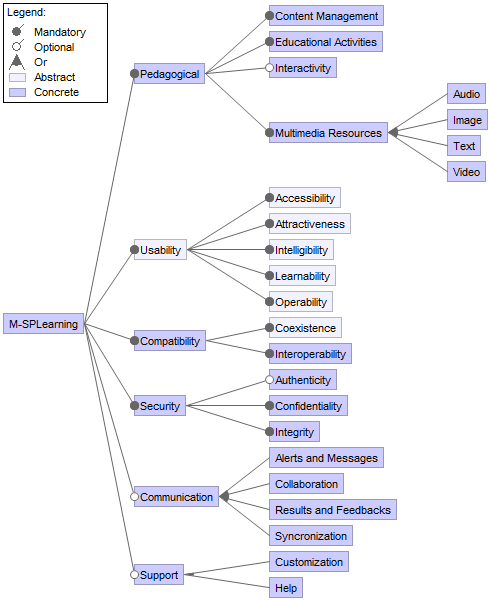
\includegraphics[width=0.91\textwidth]{MSPLFeatureModel.png}
\centering
\caption{\texttt{M-SPLear\allowbreak ning}: Feature Model.}
\label{fig:msplearning-fm}
\end{figure*}

Besides that, to standardize the variability management, SMarty was used in all the diagrams modeled for the \texttt{M-SPLear\allowbreak ning}: Architecture , Components Design and Production Plan. In this sense, one of its most representative assets is the architecture diagram (Figure \ref{fig:msplearning-architecture}). This diagram is the main artifact of the Architecture phase, because it presents the variabilities, commonalities and interactions between the SPL architectural components. Therefore, we have an overview of the product line and its domain modeling, essential information for the Design phase that details the responsibility of each component.

\begin{figure*}[!htbp]
\centering
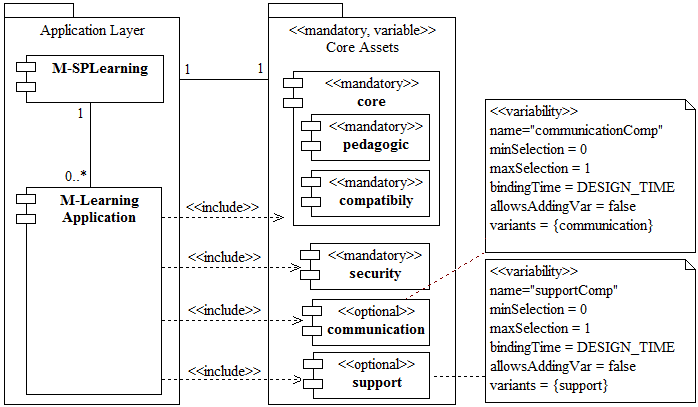
\includegraphics[width=0.92\textwidth]{MSPLArchitecture.png}
\centering
\caption{\texttt{M-SPLear\allowbreak ning}: Architecture (SMarty-based Component Diagram).}
\label{fig:msplearning-architecture}
\end{figure*}

Finally, with the support of these approaches and tools it was possible to instantiate our SPL, allowing an experimental evaluation of its products. In this sense, the Figure \ref{fig:msplearning-web} presents \texttt{M-SPLear\allowbreak ning}'s creation page, with the selection of variabilities for product generation. The following section details how the experiment was conducted to evaluate these products.

\begin{figure*}[!htbp]
\centering
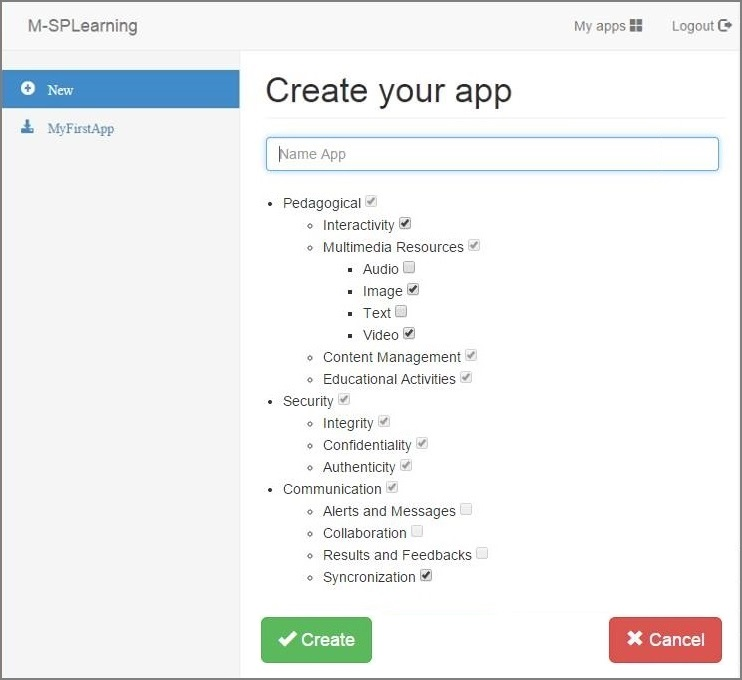
\includegraphics[width=0.75\textwidth]{MSPLWebGeneration.jpg}
\centering
\caption{\texttt{M-SPLear\allowbreak ning}: Product creation page.}
\label{fig:msplearning-web}
\end{figure*}


%TODO [OK] Sugestão: "Diluir" o  Background na Introducão para ter mais espaco para a M-SPLearning. Além disso, reduzir a secão de Trabalhos Relacionados (3 ou 4 parágrafos somente).
